\subsection{Hi-fi prototyping}\label{subsec:hi-fi-prototyping}

During the course of the hackathon week, the group also made a high-fidelity prototype~\cite{hi-lo-fidelity}.
This prototype was made within the software solution itself, but without logic behind it and with mock data.
Doing this allowed for an easier transition from the prototype to the final product.
It also represented a more accurate experience of the final product, which made it easier to test and evaluate.

The hi-fi prototype, which can be seen in Figure~\ref{fig:hifi-prototype} is similar to the lo-fi prototype, but with a
more polished look.
The look of the charts is very close to the final design, minus a few minor changes that were made after the group
received feedback for the prototype.
This iteration does not communicate with the back-end, so the data is static.
It is also impossible to filter the data using the calendar view, as this feature would require a database connection.

The group could not implement the feedback they got for the lo-fi prototype, as the hi-fi prototype was made before
the feedback was received.
Instead, the feedback was used to improve the final design.
The examples in the figure include the bar chart and heatmap as seen in Figure~\ref{subfig:hifi-bar}
and~\ref{subfig:hifi-heatmap} respectively.
These are again both components that show the user some data.

\begin{figure}[H]
    \centering
    \begin{subfigure}{.75\textwidth}
        \centering
        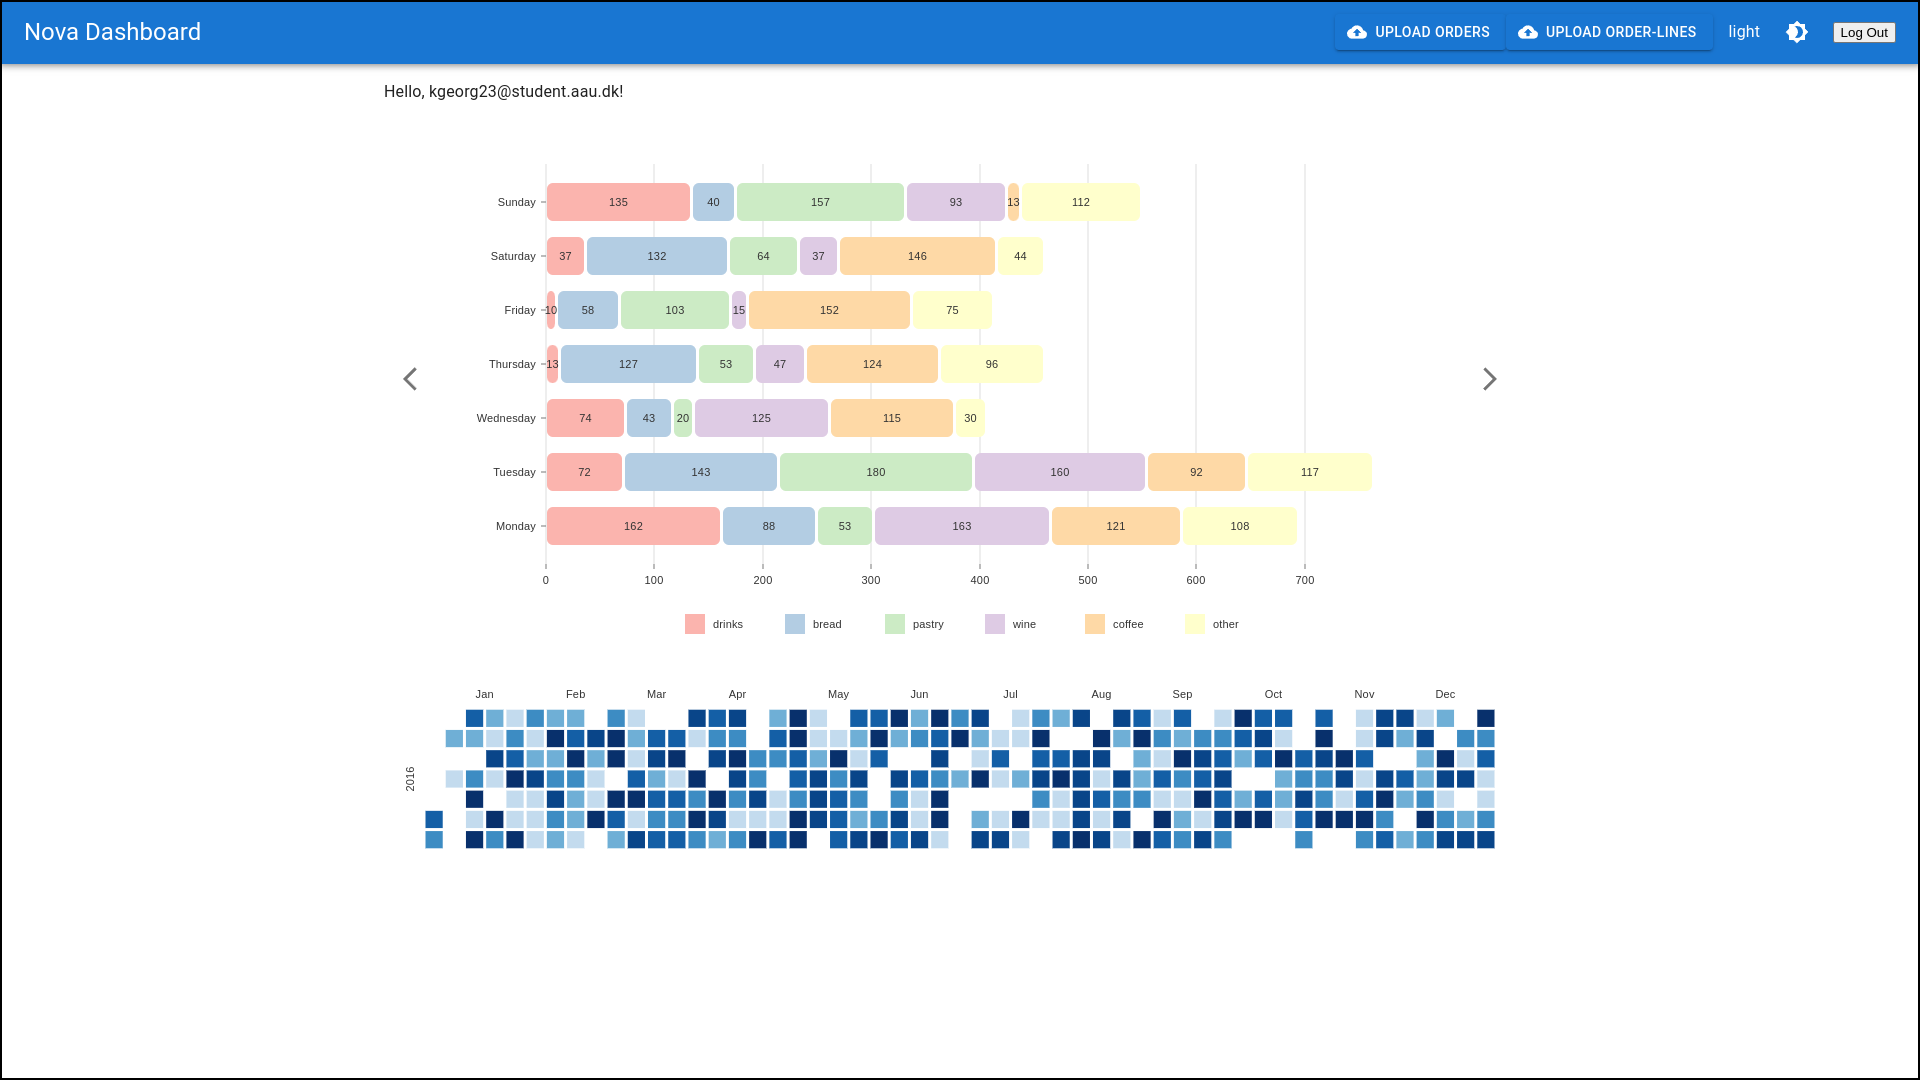
\includegraphics[width=\linewidth]{design-hifi-bar}
        \caption{Bar chart.
        }\label{subfig:hifi-bar}
    \end{subfigure}
    \par\medskip
    \begin{subfigure}{.75\textwidth}
        \centering
        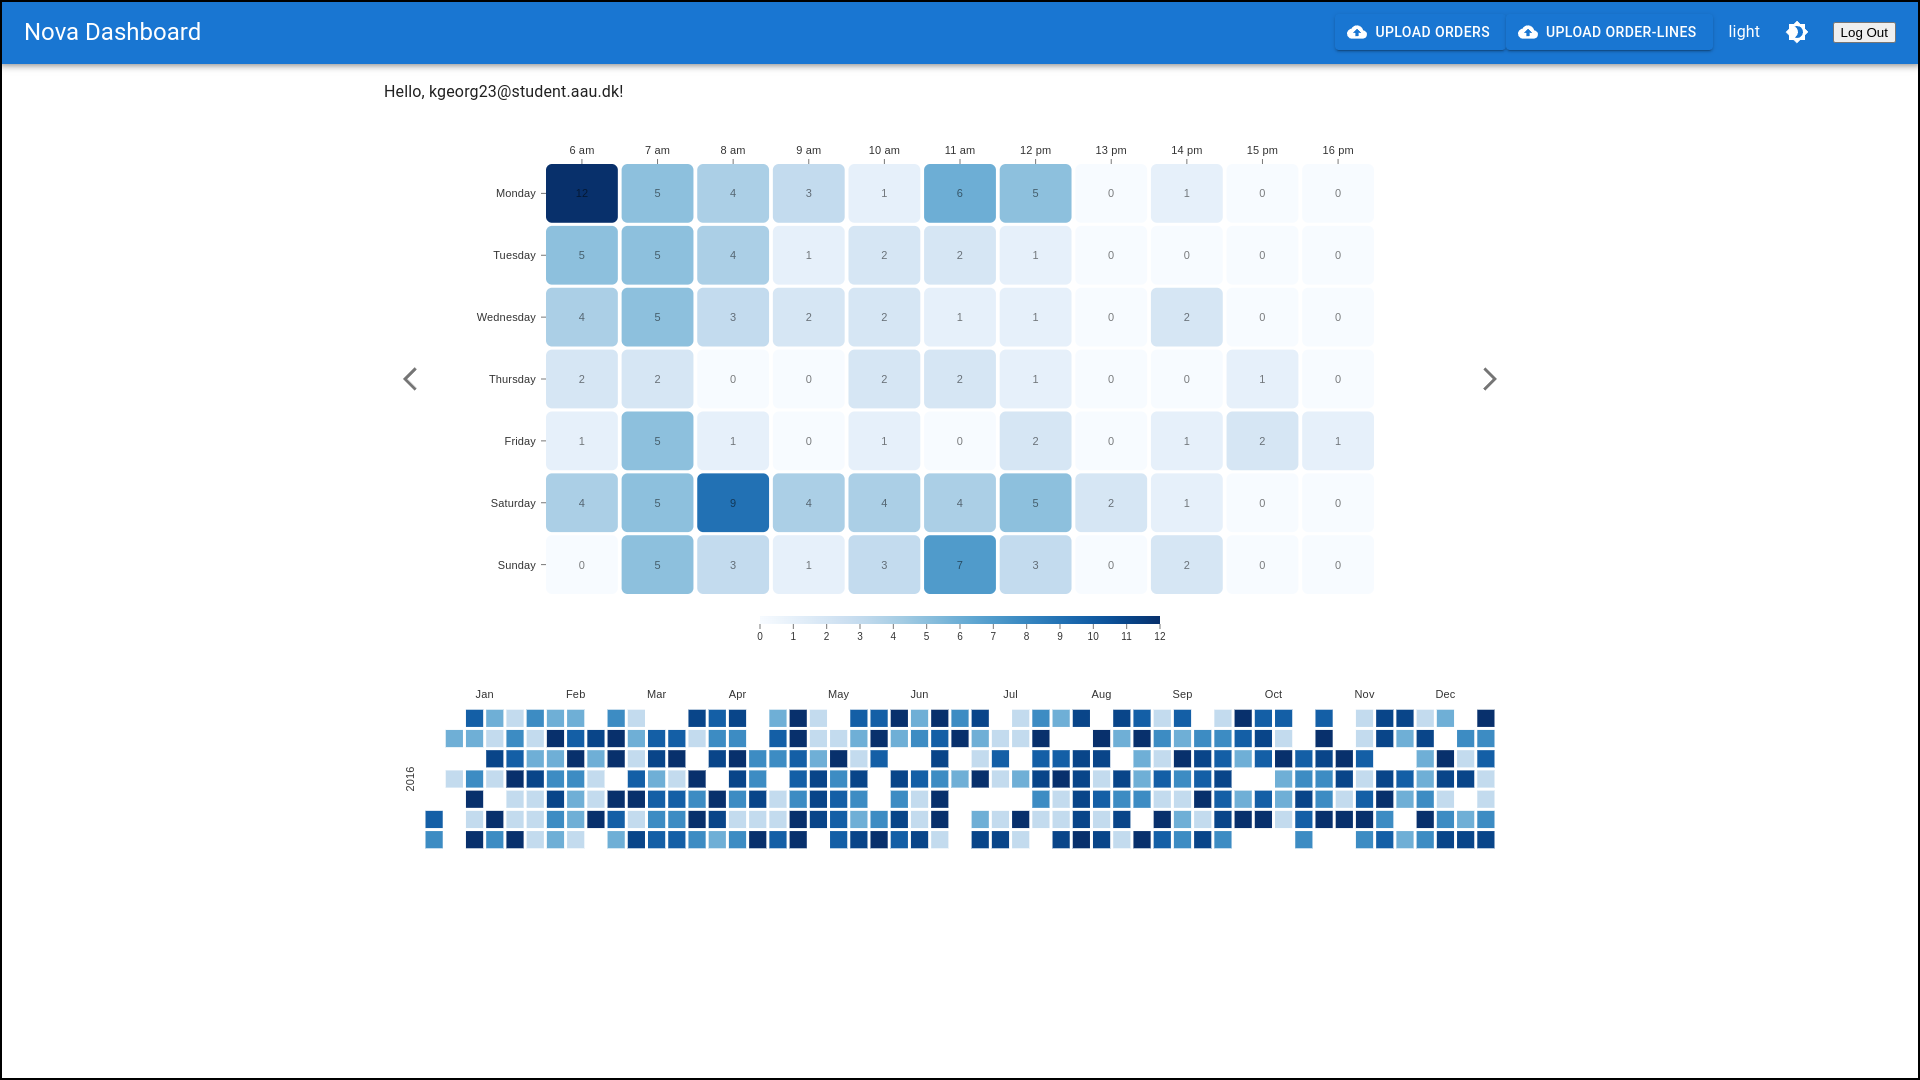
\includegraphics[width=\linewidth]{design-hifi-heatmap}
        \caption{Heatmap.
        }\label{subfig:hifi-heatmap}
    \end{subfigure}
    \caption{Hi-fi prototype.
    }\label{fig:hifi-prototype}
\end{figure}
